\documentclass{article}
\usepackage[14pt]{extsizes} % для того чтобы задать нестандартный 14-ый размер шрифта
%\usepackage[utf8]{inputenc}
\usepackage{mathtext}
\usepackage[english, russian]{babel}
%\usepackage{pscyr}(????)
\usepackage{amsmath}
\usepackage{amsfonts}
%\usepackage{setspace,amsmath}
\usepackage[left=15mm, top=15mm, right=12mm, bottom=15mm, nohead, footskip=10mm]{geometry} % настройки полей документа
\usepackage{graphicx}
\usepackage{wrapfig}
\usepackage{placeins}
\usepackage[T2A]{fontenc}			% кодировка
\usepackage[utf8]{inputenc}			% кодировка исходного текста

\begin{document}
\title{Лабораторная работа 4.3.2  \\
"Дифракция света на ультразвуковой волне в жидкости"}
\maketitle
	\paragraph*{Цель работы:} изучение дифракции света на синусоидальной акустической решетке и
	наблюдение фазовой решетки методом темного поля.
	
	\paragraph*{Оборудование:} оптическая скамья, осветитель, два длиннофокусных объектива, кювета с жидкостью, кварцевый излучатель с микрометрическим винтом, генератор звуковой частоты, линза, вертикальная нить на рейтере, микроскоп.
	
	\section{Теоретическое введение}
	
	В работе используются оптическая скамья, осветитель, два длиннофокусных объектива, кювета с жидкостью, кварцевый излучатель с микрометрическим винтом, генератор звуковой частоты, линза, горизонтальная нить на рейтере, микроскоп. 
	
	При прохождении ультразвуковой волны через жидкость в ней возникают периодические неоднородности коэффициента преломления, создается фазовая решетка, которую мы считаем неподвижной ввиду малости скорости звука относительно скорости света. Показатель
	преломления n изменяется по закону:
	
	\begin{equation}\label{}
	n = n_0 (1 + m \cos \Omega x)
	\end{equation}
	
	Здесь $ \Omega = 2 \pi / \Lambda $ --- волновое число для ультразвуковой волны, $ m $ --- глубина модуляции $ n $ $ (m \ll 1 $).
	
	Положим фазу $ \phi $ колебаний световой волны на передней стенке кюветы равной нулю, тогда на задней поверхности она равна:
	
	\begin{equation}\label{}
	\phi  = k n L = \phi_0 (1 + m \cos \Omega x)
	\end{equation}
	
	Здесь $ L $ --- толщина жидкости в кювете, $ k = 2 \pi / \lambda $ --- волновое число для света.
	
	После прохождения через кювету световое поле есть совокупность плоских волн, распространяющихся под углами $ \theta $, соответствующими максимумам в дифракции Фраунгофера:
	
\begin{equation}\label{}	
	\Lambda \sin \theta_m = m \lambda
\end{equation}

	\begin{figure}[h!]
		\centering	
		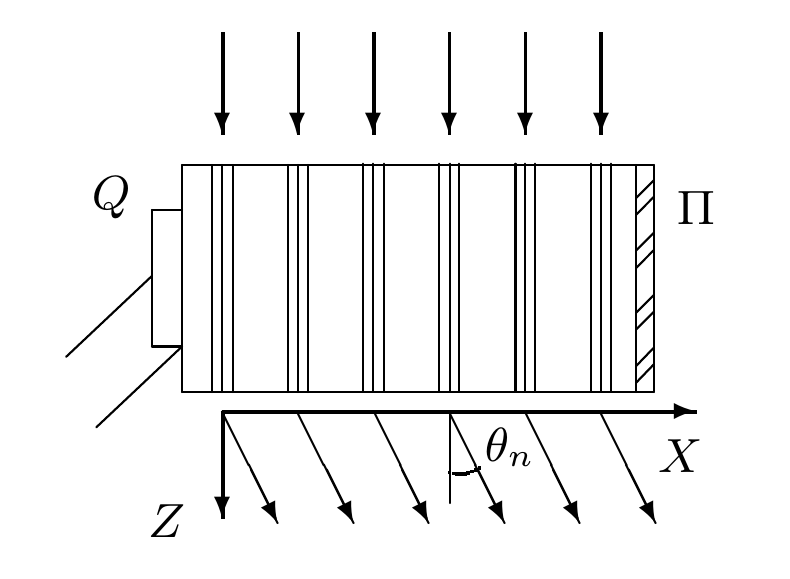
\includegraphics[width=0.3\textwidth]{difraction.png}
		\caption{Дифракция световых волн на акустической решетке}
	\end{figure}

	Зная положение дифракционных максимумов, по формуле (1) легко определить длину ультразвуковой волны, учитывая малость $ \theta $: $ \sin \theta \approx \theta \approx l_m /F  $, где $ l_m $ --- расстояние от нулевого до последнего видимого максимума, $ F $ --- фокусное расстояние линзы. Тогда получим:
	
	\begin{equation}\label{}
	 \Lambda = m \lambda F/ l_m 
	\end{equation}
	Скорость ультразвуковых волн в жидкости, где $ \nu $ --- частота колебаний излучателя:
	
\begin{equation}\label{}
	v = \Lambda \nu 
\end{equation}
\section*{Определение скорости ультразвука по дифракционной картине}
\begin{figure}[h!]
	\centering	
	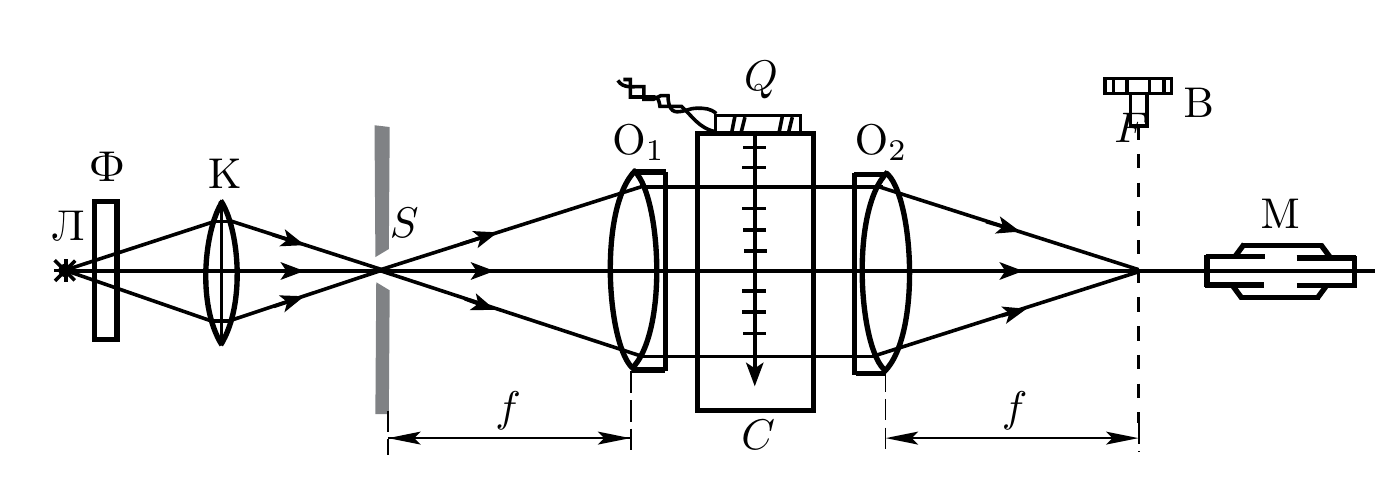
\includegraphics[width=0.7\textwidth]{shema1.png}
	\caption{Схема для наблюдения дифракции на акустической решетке}
	\label{shema1}
\end{figure}
\newpage
Измерим координаты полос для разных частот:
\begin{table}[h!]
\begin{tabular}{|l|l|l|l|l|l|l|l|l|l|l|l|l|l|l|l|l|}
\hline
$\nu$, МГц         & \multicolumn{5}{l|}{1.3}   & \multicolumn{3}{l|}{2} & \multicolumn{3}{l|}{4.3} & \multicolumn{5}{l|}{1} \\ \hline
$m$ & -2  & -1  & 0   & 1   & 2  & -1     & 0      & 1    & -1      & 0      & 1     & -2  & -1  & 0   & 1   & 2  \\ \hline
$x_m$, 4мкм      & 224 & 180 & 142 & 101 & 62 & 210    & 150    & 85   & 279     & 146    & 13    & 220 & 178 & 145 & 114 & 85 \\ \hline
\end{tabular}
\end{table}
\\
Построим графики для разных частот и по углу наклона найдем $l_m/m$
\begin{figure}[h!]
	\centering	
	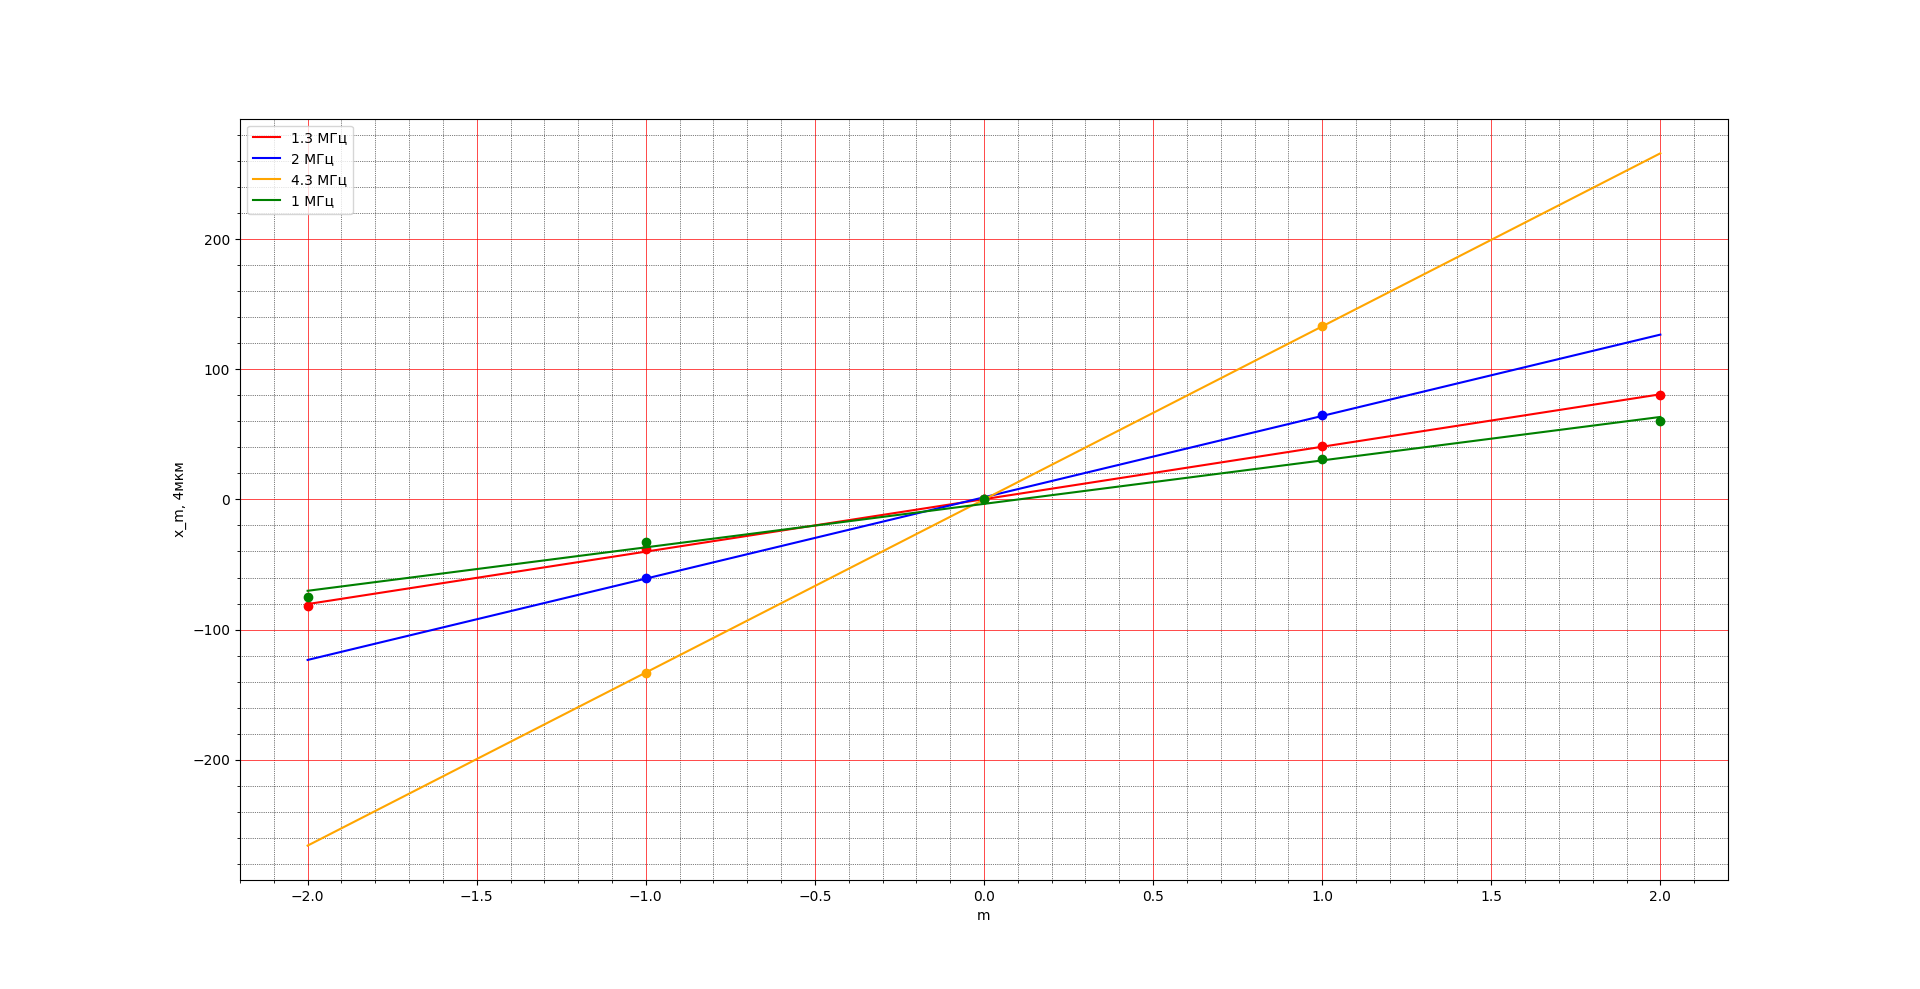
\includegraphics[width=1\textwidth]{Laba_432_grath1.png}
	\caption{максимумы для разных частот}
	\label{Laba_432_grath1.png}
\end{figure}
\\
В итоге мы знаем параметры установуки: $F=28 ~ см$. Возьмем $\lambda = (6400 \pm 200) ~ A$ и $\sigma_x=12 ~ мкм$ 
и с помощью формул $l_m= {mf\lambda \over 
\Lambda}$, $v=\Lambda\nu $ расчитаем скорость звука
\begin{table}[h!]
\centering
\begin{tabular}{|l|l|l|l|l|l|}
\hline
$\nu ~ МГц$  & ${x_m\over m} ~ мкм$ & $\Lambda~мм$   & $\sigma_\Lambda~мм$     & $v ~ {м \over c}$      & $\sigma_v$         \\ \hline
1.3          & 40.3                     & 1.11           & 0.04               & 1450                       & 60               \\ \hline
2            & 62.5                     & 0.71           & 0.03               & 1430                       & 60              \\ \hline
4.3          & 133                      & 0.34           & 0.02               & 1450                       & 60              \\ \hline
1            & 33.4                     & 1.34           & 0.05               & 1340                       & 50               \\ \hline
\end{tabular}
\end{table}  
\\ Таким образом взяв среднее получим конечный результат:
$$v=(1420 \pm 70) ~ {м \over с}$$
\newpage
\section*{Определение скорости ультразвука методом темного поля}
\begin{figure}[h!]
	\centering	
	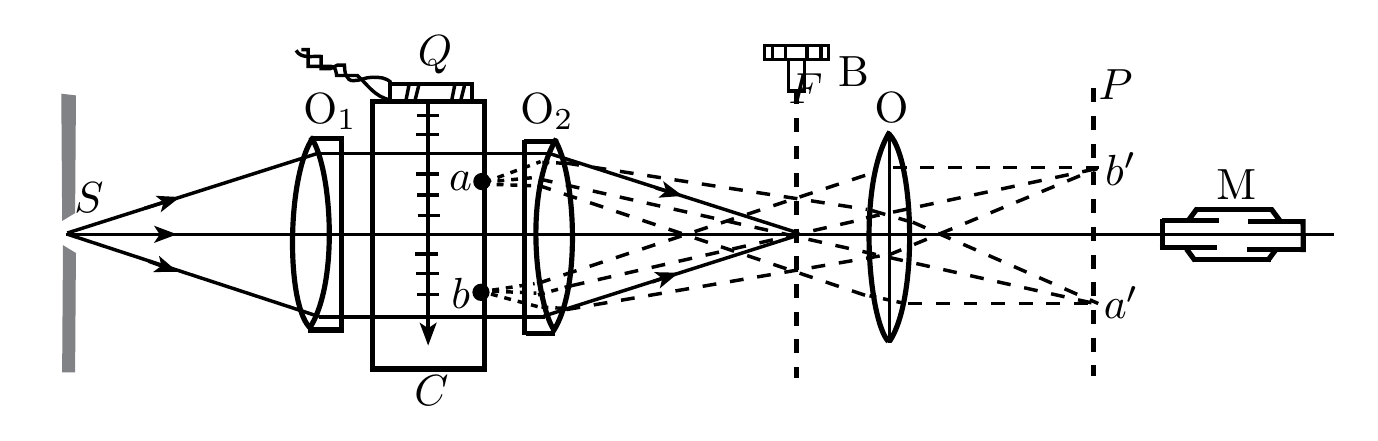
\includegraphics[width=0.7\textwidth]{shema2.png}
	\caption{Схема для наблюдения дифракции методом темного поля}
	\label{shema2}
\end{figure}

С помощью калибровочной сетки найдем что при измерении длины волны нужно считать для микроскопа $1 ~ ед. ~ изм. = (2.4 \pm 0.1) ~ мм$
померим зависимость длины волны от частоты
\begin{table}[h!]
\centering
\begin{tabular}{|l|l|l|l|l|l|}
\hline
$\nu$ & $y_1$ & $y_2$ & n  & $\Lambda$        & $\sigma_\Lambda$  \\ \hline
2     & 0.6   & 2.5   & 12 & 15.8             & 0.6 \\ \hline
1.14  & 2.9  & 1.0    & 7  & 23               & 1             \\ \hline
1.04  & 2.9  & 1.0    & 6  & 26               & 1  \\ \hline
0.98  & 1.0  & 3.1    & 7  & 36.2             & 1.4   \\ \hline
1.34  & 1.1   & 2.5   & 6  & 20               & 0.8               \\ \hline
\end{tabular}
\end{table}
\\
теперь с помощью графика $\Lambda({1 \over \nu})$ найдем v
\begin{figure}[h!]
	\centering	
	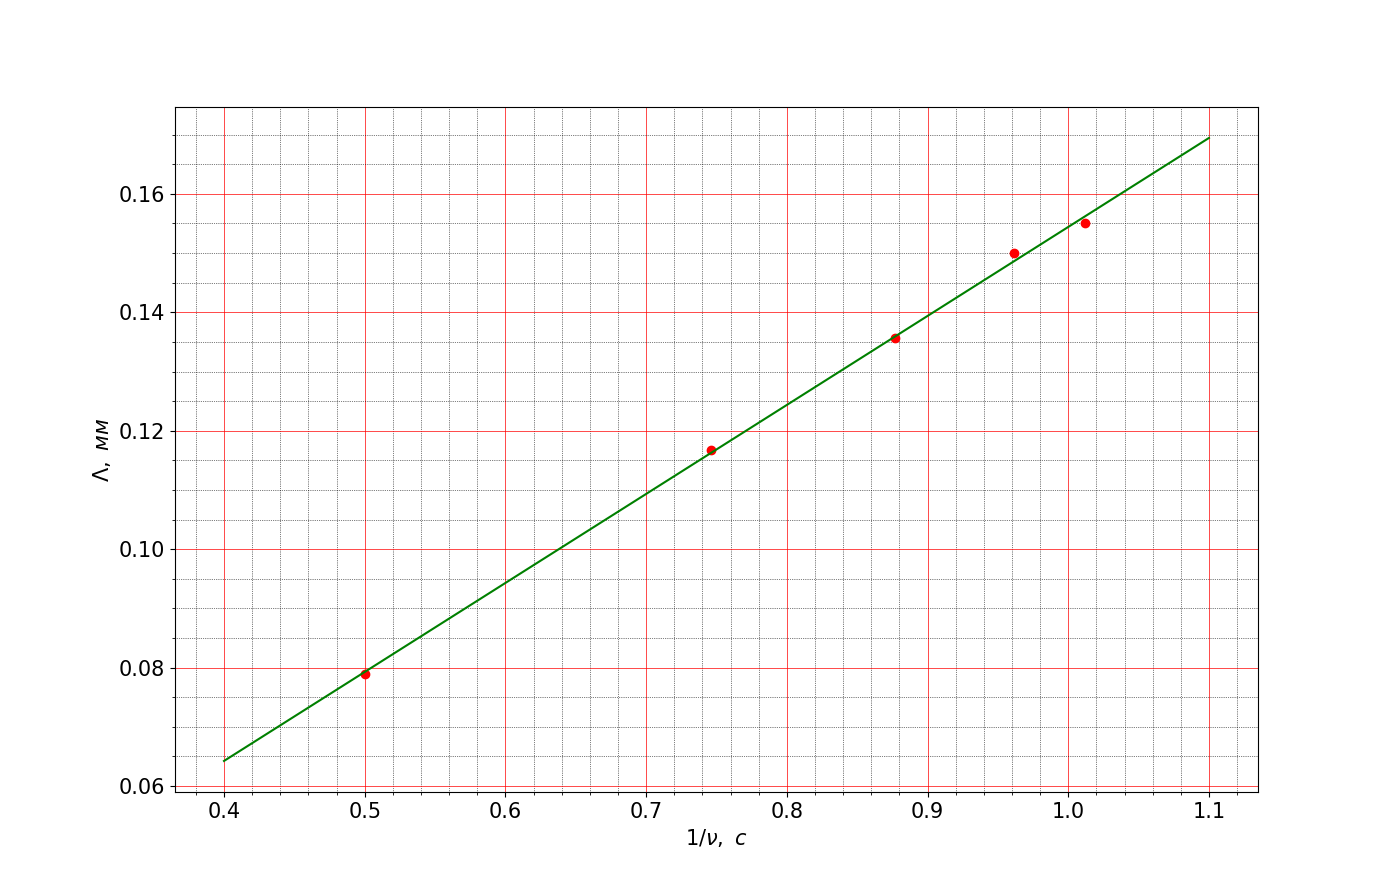
\includegraphics[width=0.6\textwidth]{Laba_432_grath2.png}
	\caption{максимумы для разных частот}
	\label{Laba_432_grath2.png}
\end{figure}
\\
Таким образом $v=(1500 \pm 60) ~ {м \over с}$
\section*{Вывод}
Мы с неплохой точностью померили длину звуковой волны в жидкости, в сборнике физических величин $v_{табл}=1482$, также изучили метод темного поля.
\end{document}
